\documentclass{article}
\title{ECE 370 -- Homework 2}
\usepackage[margin=1in]{geometry}
\usepackage{graphicx}
\usepackage{pdfpages}
\usepackage{fancyhdr}
\usepackage{enumitem}
\usepackage{pdfpages}
\usepackage{amsmath}
\usepackage{amssymb}
\usepackage{float}
\pagestyle{fancy}
\fancyhf{}
\fancyhead[L]{Gianni Avilan-Losee}
\fancyhead[C]{ECE 370}
\fancyhead[R]{Homework 2}
\fancyfoot[C]{\thepage}
\usepackage{microtype}
\usepackage{textcomp, gensymb}
\author{Gianni Avilan-Losee}
\setcounter{section}{1}
\begin{document}
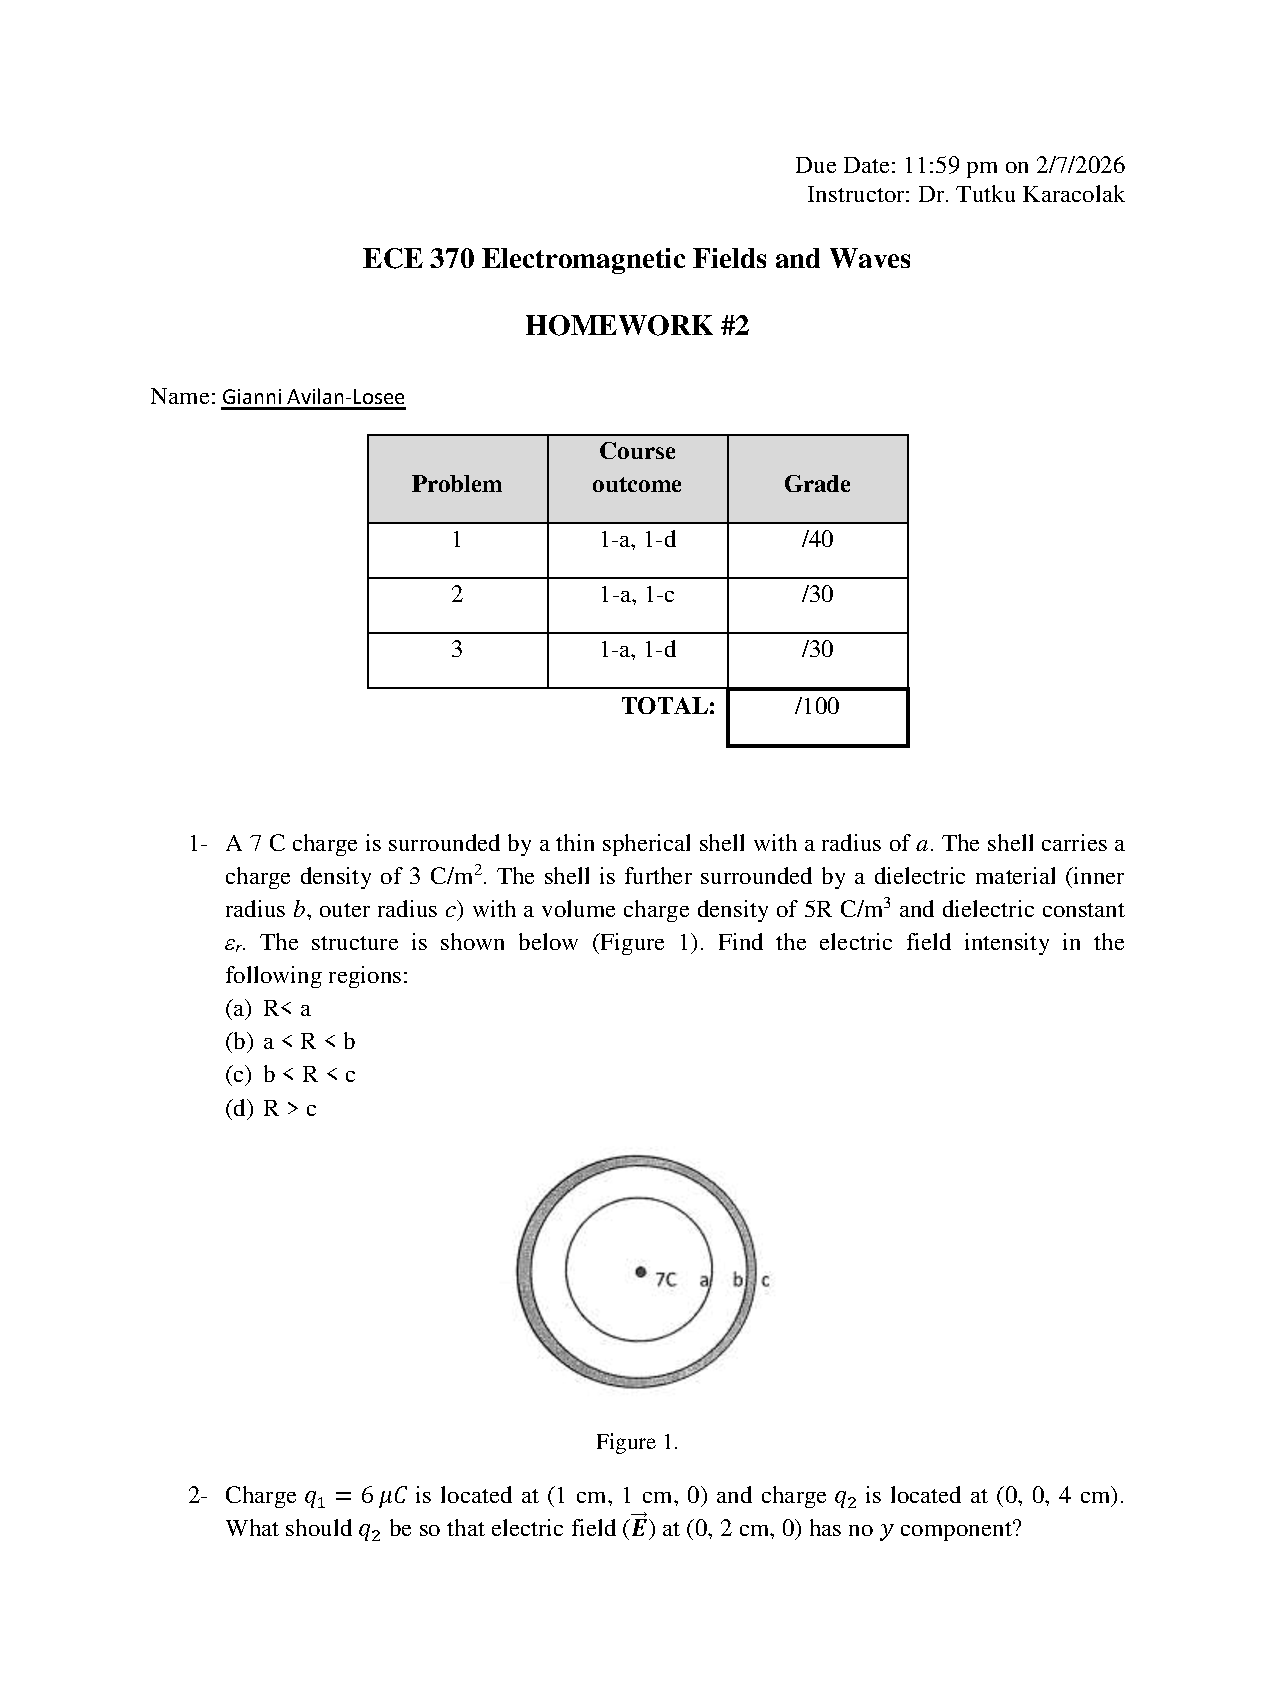
\includepdf[pages=-]{homework-2_cover-page.pdf}
\begin{enumerate}
	\item Here, a spherical Gaussian surface seems the most useful tool, since we may then enclose all the given charge in the problem as the radius of the Gaussian sphere grows, and use Gauss's Law, \[
	  \oint_{S}\vec{D} \cdot d \vec{s} = Q,
	\]
  to determine the net total intensity of the electric field at any point \(P\), at a distance of \(R\) from the origin.

	Placing the \(7\mathrm{C}\) point at the origin and using spherical coordinates, we may then simplify Gauss's Law in this case to \[
		E \int_{0}^{2\pi}\int_{0}^{\pi} R^2 \sin{(\theta)} \ d\theta \ d\phi = \frac{Q}{\varepsilon} \Rightarrow E = \frac{1}{4\pi\varepsilon} \ \frac{Q}{R^2}, 
	\]
	where \(\varepsilon\) represents the electric permittivity of the medium in which \(P\) is placed and \(Q\) represents the total charge enclosed by the Gaussian sphere of radius \(R\). Unless otherwise noted, the electrical permittivity \(\varepsilon = \varepsilon_{0}\), the electrical permitivitty of free space. 

	Additionally, due to the symmetric properties of the charged spheres given in the problem, no net electric field is generated by the charged spheres within the bounds of their inner radii, and we assume the total electric field generated at their surfaces is parallel to the radial unit vector \(\hat{\alpha_R}\).

	Given the above, we may now solve for the electric field intensity in each of the regions given in the problem by simply finding the total charge enclosed by the Gaussian sphere at a radius R. 
	\begin{enumerate}[label=\alph*)]
		\item In the first case, where \(R < a\) and the electrical permittivity of the medium is assumed to be \(\varepsilon_{0}\), the total charge enclosed by the Gaussian surface is \(Q = 7\mathrm{C}\), and so Gauss's Law shows that \[
				E(R) = \frac{7}{4\pi\varepsilon_{0}R^2} \ \mathrm{\frac{V}{C}}.
		\]
	\item In the second case, where \(a < R < b\), we may find the total charge enclosed by the Gaussian surface by summing the previous charge with the total charge contained on the first charged sphere's surface, given by the sphere's charge density times its area, \(\rho_{s} 4\pi a^2 = 12\pi a^2\). (We could also derive this using a surface integral, but since the charge density is uniform, it's simpler to use the formula for the surface area of a sphere).

		Then, the electric field intensity in this region is given by \[
			E(R) = \frac{7+12\pi a^2}{4\pi\varepsilon_{0}R^2} \ \mathrm{\frac{V}{C}}.
		\]
	\item Next, in the region \(b < R < c\), total charge depends on the radius and increases linearly from \(R = b\) to \(R = c\). Here, we may use a volume integral to find the charge as a function of \(R\), \[
			Q(R) = \int_{0}^{2\pi}\int_{0}^{\pi}\int_{b}^{R}\rho_{v}R^2\sin{(\theta)} \ dR \ d\theta \ d\phi = 5\pi(R^4-b^4) \ \mathrm{C}.
	\]

	We may then include this new volume charge in our sum; however, the electrical permittivity in the region is now \(\varepsilon_r\), and so \[
		E(R) = \frac{7+12\pi a^2 + 5\pi(R^4-b^4)}{4\pi\varepsilon_rR^2} \ \mathrm{\frac{V}{C}}.
	\]
    \item Finally, in the region defined by \(R > c\), we may include the entire volume charge enclosed by the dielectric shell from \(b\) to \(c\), \[
				Q = \int_{0}^{2\pi}\int_{0}^{\pi}\int_{b}^{c}\rho_vR^2\sin{(\theta)} \ dR \ d\theta \ d\phi = 5\pi(c^4-b^4) \ \mathrm{C}.
    \]

		Summing all charges and returning to a region with vaccum permittivity, the electric field intensity is given by \[
			E(R) = \frac{7+12\pi a^2 + 5\pi(c^4-b^4)}{4\pi\varepsilon_0R^2} \ \mathrm{\frac{V}{C}}.
		\]
	\end{enumerate}
\item To calculate the electric field vector induced by two point charges, Coulomb's Law, \[
		\vec{E} = \frac{q}{4\pi\varepsilon_0R^2} \ \hat{\alpha_R} \ \mathrm{\frac{V}{C}}
\]
  is the most convenient tool available.
	
	Since Coloumb's Law expresses field in terms of the radial distance from the source of charge, we may first find the magnitude of the difference vectors between the given point \(P\) and the two charges \(q_1\) and \(q_2\) as \begin{align*}
		&R_1 = \sqrt{-0.01^2+0.01^2} = 0.0141 \ \mathrm{m}, \\
		&R_2 = \sqrt{0.02^2 + (-0.04)^2} = 0.0447 \ \mathrm{m},
	\end{align*} 
	and their unit vectors as \begin{align*}
	 & \hat{\alpha_{R1}} = \frac{(-0.01, 0.01, 0)}{0.0141} = (-\frac{1}{\sqrt{2}}, \frac{1}{\sqrt{2}}, 0), \\
	 & \hat{\alpha_{R2}} = \frac{(0, 0.02, 0.04)}{0.0447} = (0, \frac{2}{\sqrt{20}}, -\frac{4}{\sqrt{20}}).
	\end{align*} 
	Then, multiplying magnitude and direction together, we may find the electric field vector induced by each point charge as \begin{align*}
		&\vec{E}_1 = \frac{6 \times 10^{-6}}{4 \pi (8.85 \times 10^{-12})(1.988 \times 10^{-4})} \ \hat{\alpha_{R1}}=(-1.919 \times 10^8, 1.919 \times 10^8, 0) \ \mathrm{\frac{V}{C}},  \\
		&\vec{E}_2 = \frac{q_2}{4 \pi (8.85 \times 10^{-12})(0.002)} \ \hat{\alpha_R} = (0, q_2 2.013 \times 10^{12}, q_2 4.03 \times 10^{12}) \ \mathrm{\frac{V}{C}}.
	\end{align*} 
	Then, focusing just on the y-components of the fields, \[
		q_2 2.013 \times 10^{12} - 1.919 \times 10^8 = 0 \Rightarrow q_2 = \frac{-1.919 \times 10^8}{2.013 \times 10^{12}} = -95.33 \micro\mathrm{C}. 
	\] 
	\item Similarly to the first problem, we may find the charge contained on both spherical surfaces and use Gauss's Law to find the resultant electric field. 
		
		In the region \(R<a\), no electric field exists due to the symmetrical properties of the sphere (like charges cancel each other out). 

		In the region \(a < R < b\), the electric field is given by \[
			\vec{E} = \frac{Q_1}{4\pi\varepsilon_0R^2} \ \hat{\alpha_R} \ \mathrm{\frac{V}{C}},
		\]
		assuming vaccum permittivity, since all the charge enclosed by a Gaussian surface with radius \(a < R < b\) is equal to the charge contained on the surface of the sphere with radius \(a\), and all the electric field components point away from the sphere's surface entirely. 

		In the region \(R > b\), the Gaussian sphere used in the previous step encloses both surface charges \(Q_1\) and \(Q_2\), and so \[
			\vec{E} = \frac{Q_1+Q_2}{4\pi\varepsilon_0R^2} \ \hat{\alpha_R} \ \mathrm{\frac{V}{C}}. 
		\]
\end{enumerate}
\end{document}
